%=========================================================================
% Start of
%=========================================================================
\preClass{Basic Trigonometry}

\begin{problem}
\item A circle of radius $r$ is centered at the origin, and a ray
  originates from the origin at a given angle, $\theta$. The ray
  passes through the circle at the coordinate $(x,y)$. A function of
  $\theta$ can be defined in terms of the coordinate.

  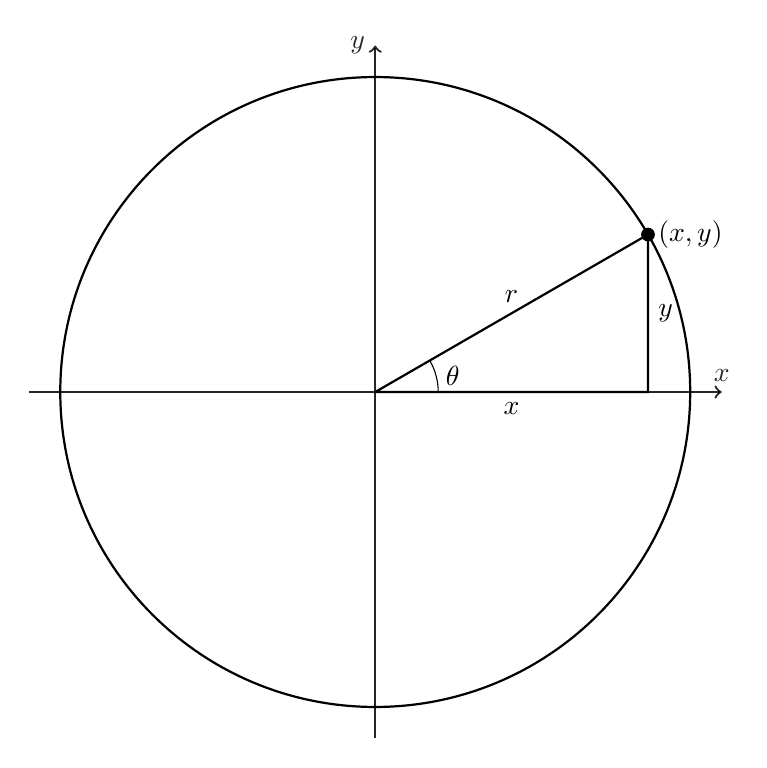
\begin{tikzpicture}[y=4cm, x=4cm,font=\sffamily]
      \draw[thick,opacity=0.85,->] (0, -1.1) -- (0,1.1) node[anchor=east] {$y$};
      \draw[thick,opacity=0.85,->] (-1.1, 0) -- (1.1,0) node[anchor=south] {$x$};
      \draw[thick] (1,0) arc (0:360:1);
      \draw[thick] (0,0) -- (30:1) node[midway,anchor=south] {$r$}
          node[anchor=west] {$(x,y)$}
          -- ++(-90:0.5) node[midway,anchor=west] {$y$}
          -- (0,0) node[midway,anchor=north] {$x$};
      \draw[fill=black] (30:1) circle (0.02);
      \draw[text=black] (0:0.2) arc (0:30:0.2) node[midway,anchor=west] {$\theta$};
    \end{tikzpicture}


  \begin{subproblem}
  \item A function, sine, is defined to be
    \begin{eqnarray*}
      \sin(\theta) & = & \frac{y}{r}.
    \end{eqnarray*}
    Determine the formula for the value of $y$ given $r$ and $\theta$
    in terms of the sine function.
    \sideNote{Solve the equation above for $y$.}
    \vfill
  \item A function, cosine, is defined to be
    \begin{eqnarray*}
      \cos(\theta) & = & \frac{x}{r}.
    \end{eqnarray*}
    Determine the formula for the value of $x$ given $r$ and $\theta$
    in terms of the cosine function.
    \sideNote{Solve the equation above for $x$.}
    \vfill
  \end{subproblem}

\end{problem}


\actTitle{Basic Trigonomety}
\begin{problem}
\item Answer each of the following questions where the given point is $P(2,4)$.
  \begin{subproblem}
  \item Make a sketch of the coordinate plane and include the point
    $P(2,4)$. Draw the ray from the origin to the point.
    \sideNote{Label your axes and annotate your plot.}
    \vfill
  \item Add a circle to your sketch whose center is the origin and goes
    through the point. Label the angle $\theta$ as the angle between
    the ray and the $x$-axis.
  \item What is the radius of the circle? (Add a label to your plot for the radius.)
    \vspace{2em}
  \item Determine the values of the sine and cosine for the angle.
    \begin{eqnarray*}
      \sin(\theta) & = & \\ [10pt]
      \cos(\theta) & = &
    \end{eqnarray*}
  \end{subproblem}

\clearpage

\item Different points are given below. For each point assume it is
  on the edge of a circle whose center is at the origin.
  Determine the radius of the circle as well as the value of the
  sine and cosine of the angle associated with each point on its circle.
  \begin{subproblem}
  \item $P(1,0)$
    \vfill
  \item $P(0,1)$
    \vfill
  \item $P(-1,0)$
    \vfill
  \item $P(0,-1)$
    \vfill
  \item $P\left(\frac{\sqrt{2}}{2},\frac{\sqrt{2}}{2}\right)$
    \vfill
  \end{subproblem}

\clearpage

\item In each item below some information is given about an angle.
  Use the information to determine the sine, cosine, and tangent of the
  angle. In each case determine if the sine, cosine, and tangent will
  increase or decrease if the angle is increased by a small amount.
  \begin{subproblem}
    \item The angle is in the first quadrant and $\cos(\theta)=0.3$.
      \vfill
    \item The angle is in the third quadrant and $\sin(\theta)=-0.25$.
      \vfill
    \item The angle is in the second quadrant and $\cos(\theta)=-0.8$.
      \vfill
  \end{subproblem}

  \clearpage

  \item An airplane is observed, and it is flying directly away from an observer
    in level flight.
    The observer measures the angle of elevation for the plane at two different
    times. You wish to determine the height of the plane.
    \begin{subproblem}
      \item The plane is moving away from the observer. Will the angle increase
        or decrease?
        \vspace{2em}
      \item At the first time the angle of elevation is 20$^\circ$.
        At the second time the angle of elevation is 13$^\circ$.
        It is estimated that the plane flew a distance of 3 miles between observations.
        Draw a rough sketch of the situation.
        \sideNote{You should have two triangles.}
        \vfill
        \item Determine the number of unknowns and determine how many equations you need.
          \vspace{1em}
      \item Determine a relevant formula each of the two triangles plus any
        other equations you may need.
        \vfill
      \item Solve the system of equations to determine the height of the plane.
        \vfill
        \vfill
    \end{subproblem}

\end{problem}

\postClass

\begin{problem}
\item Briefly state two ideas from today's class.
  \begin{itemize}
  \item
  \item
  \end{itemize}
  \item The circle below is centered at the origin and has a radius of
    one.

    %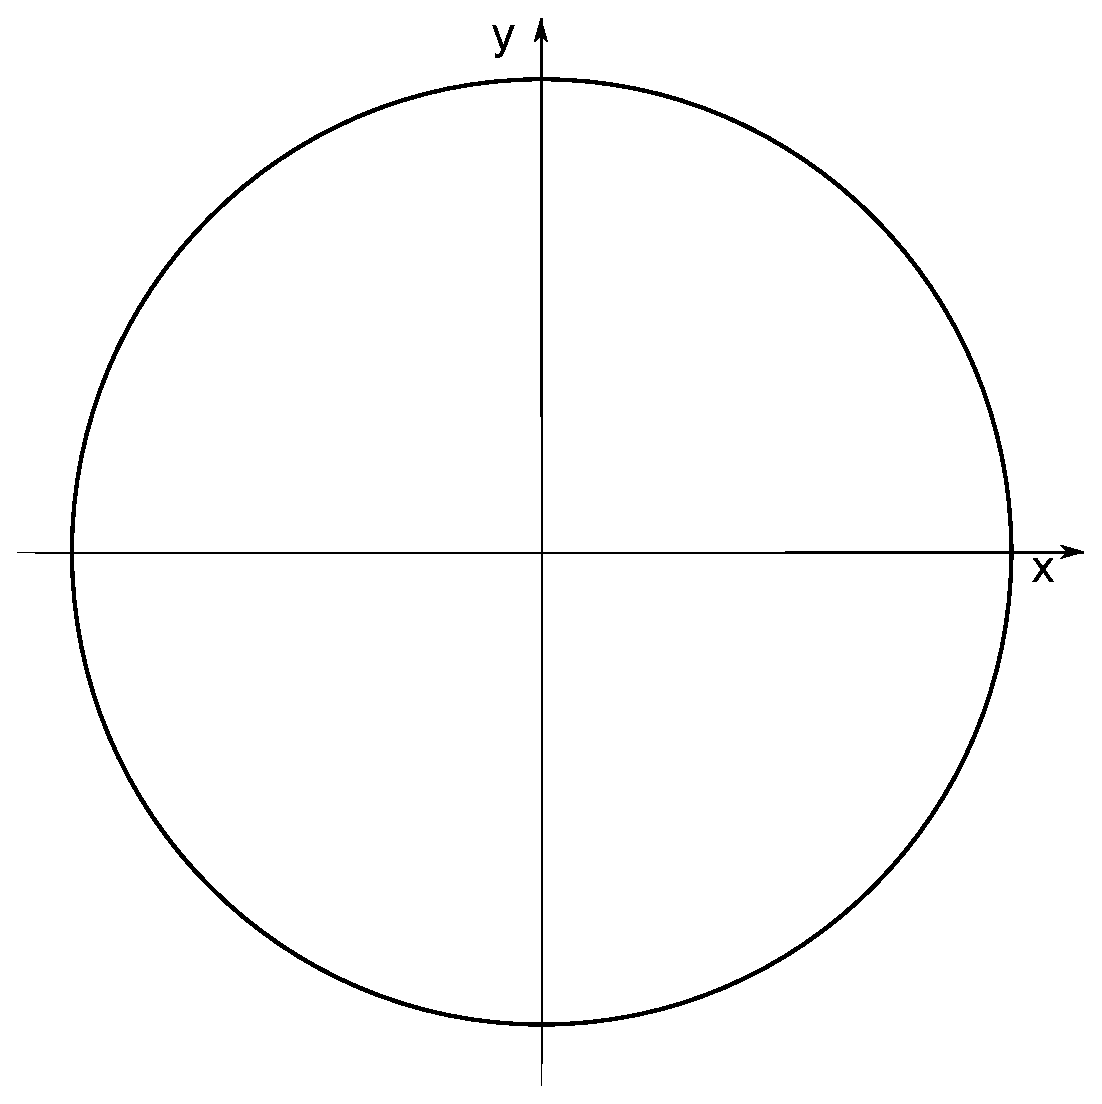
\includegraphics[width=16cm]{trig/img/blankCircle}
    \begin{tikzpicture}[y=6cm, x=6cm,font=\sffamily]
        \draw[thick,opacity=0.85,->] (0, -1.1) -- (0,1.1) node[anchor=east] {$y$};
        \draw[thick,opacity=0.85,->] (-1.1, 0) -- (1.1,0) node[anchor=south] {$x$};
        \draw[thick] (1,0) arc (0:360:1);
      \end{tikzpicture}

    \begin{subproblem}
    \item Mark the locations on the circle whose associated angles are
      0, $\pi/4$, $\pi/2$, $3\pi/4$, $\pi$, $5\pi/4$, $3\pi/2$, and
      $7\pi/4$.
      Determine the coordinates for the points.
      (Label the points and annotate your plot.)
    \item Determine the $(x,y)$ coordinates for each angle.
    \item Determine the cosine and sine of each angle.
    \end{subproblem}
  \item An airplane is observed, and it is flying directly away from an observer
      in level flight.
      The observer measures the angle of elevation for the plane at three different
      times. You wish to determine the height of the plane.
      \begin{subproblem}
        \item The plane is moving away from the observer. Will the angle increase
          or decrease?
        \item At the first time the angle of elevation is 20$^\circ$.
          At the second time the angle of elevation is 13$^\circ$.
          At the third time the angle of elevation is 10$^\circ$.
          It is estimated that the plane is flying at a constant speed.
          The time between each measurement is 20 seconds, and the distance
          the plane flies between each measurement is $20\cdot v$ where $v$
          is measured in meters per second.
          Draw a rough sketch of the situation.
          \sideNote{You should have three triangles.}
          \vfill
          \item Determine the number of unknowns and determine how many equations you need.
            \vspace{1em}
          other equations you may need.
          \vfill
        \item Solve the system of equations to determine the height of the plane.
          \vfill
          \vfill
      \end{subproblem}
\end{problem}


%%% Local Variables:
%%% mode: latex
%%% TeX-master: "../labManual"
%%% End:
